\documentclass[]{article}
\usepackage{graphicx}
\begin{document}

\begin{center}
    \vspace*{1cm}

    \textbf{Question 4.}

    \vspace{0.5cm}
     Algorithms Assignment 1

    \vspace{0.15cm}

    \textbf{Faaiq Bilal} \\ 
    \textbf{23100104}
         
\end{center}

\section{Part a}
True, for all $k>5$ and $n \geq 0$, $k \cdot{n^3}$ is greater than $5n^3$. Hence $5n^3$  $ \epsilon $ $O(n^3) $ \\



\section{Part b}
True \\
This condition is true as $ 100n^2 < n^4$ for some $ n > 10 $\\
e.g. $100 \times 11^2 < k \times 11^4$ for all $ k \geq 1 $ \\
Since there exists a k, for which $100n^2 < k \cdot n^4 $ is true for all $ n \geq 0 $, $ 100n^2 $ $\epsilon $ $O(n^4)$

\section{Part c}
True \\
$ \log n^2 = 2 \log n$ \\ 
$ 2 \log n < k \cdot \log n$ for any $k > 2$ \\ 
Since there exists a k, for which $2 \log n < k $ is true for all $ n \geq 0 $, $ \log n^2 $ $\epsilon $ $O(\log n)$

\section{Part d}
True \\ 
The largest term in the above expression (once expanded) will be $ (n^2)^3 = n^6$. All other terms will be smaller. Hence, there exists a constant k for which $k \cdot n^6 $ is greater than the expression given, and the function will be $O(n^6)$\\

\newpage

\section{Part e}
True
In this part, it will be helpful to consider the bounds of the two functions. Before that, we can do some simplification. \\
$ \sqrt{n} \leq k \cdot (\log n)^3 $ \\ 
$ \sqrt[6]{n} \leq k_2 \cdot \log n $ \\
We can now compare the two functions. \\
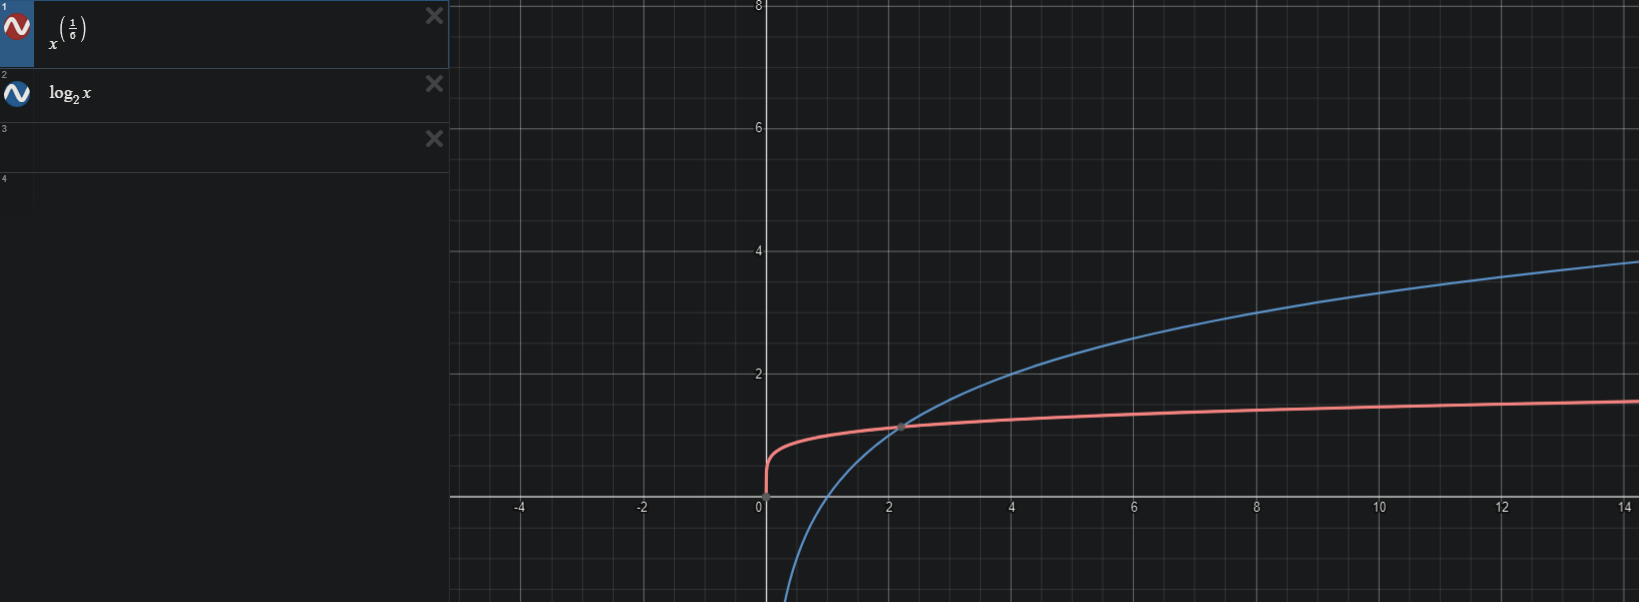
\includegraphics[scale=0.4]{Screenshot_1.png}
\\ The point of intersection is at about a value of $n=2.205$. The functions then diverge permanently, and $log n$ stays larger than $\sqrt[6]{n}$. This means that $\sqrt[6]{n} \leq k \cdot \log n$ for values of k, and all values of n larger than 2.205. 




\end{document}